\documentclass[10pt,twocolumn,twoside]{genpaper}
\usepackage[sort&compress]{natbib}

\usepackage{flushend}
\usepackage{xcolor,colortbl}
\usepackage{subfig}
\usepackage{longtable}
\definecolor{Gray}{gray}{0.9}
\newcommand{\npscarf}{$\mathtt{npScarf}$}
\newcommand{\npscarfg}{$\mathtt{npScarf\_wag}$}
\newcommand{\npreader}{$\mathtt{npReader}$}
\newcommand{\npanalysis}{$\mathtt{npAnalysis}$}
\newcommand{\npbarcode}{$\mathtt{npBarcode}$}
\newcommand{\npgraph}{$\mathtt{npGraph}$}
\newcommand{\canu}{$\mathtt{Canu}$}
\newcommand{\unicycler}{$\mathtt{Unicycler}$}
\newcommand{\spades}{$\mathtt{SPAdes}$}
\newcommand{\albacore}{$\mathtt{Albacore}$}
\newcommand{\racon}{$\mathtt{Racon}$}
\newcommand{\metrichor}{$\mathtt{Metrichor}$}
\newcommand{\minimap}{$\mathtt{minimap2}$}
\newcommand{\miniasm}{$\mathtt{miniasm}$}
\newcommand{\bwa}{$\mathtt{BWA\text{-}MEM}$}

\newcommand{\ec}{\emph{E.~coli}}
\newcommand{\sce}{\emph{S.~cerevisae}}
\newcommand{\kp}{\emph{K.~pneumoniae}} 

\newcommand{\IE}{\emph{i.e.}}
\newcommand{\EG}{\emph{e.g.}}
\newcommand{\review}[1]{\textcolor{red}{#1}}

\title{Online resolving assembly graph by long reads data}
\shorttitle{Real-time Scaffolding with Assembly graph}

%Authors
\author[1]{Son Hoang Nguyen}
\author[1,$\ast$]{Lachlan Coin}

%Affiliation
\affil[1]{Institute for Molecular Bioscience, the University of Queensland, 
St Lucia, Brisbane, QLD 4072 Australia}

\correspondingauthor{
\textsuperscript{$\ast$}
To whom correspondence should be addressed. 
E-mails: author.last@email.com,author.first@email.com
}

%To show compiled date
\compiledate

\begin{document}
%Abstract and keywords have to be defined before \maketitle

\onecolumn
\renewcommand{\figurename}{Supplementary Figure}
\renewcommand{\tablename}{Supplementary Table}
%\setcounter{page}{1}
\setcounter{figure}{0}
\setcounter{table}{0}
% 
\begin{center}
 \Large{Supplementary Information}
\end{center}


\makeatletter

\newlength\oriarrayrulewidth  
\newcount\orilowpenalty
\newcommand\nobreakmidrule{%
 \noalign{\global\oriarrayrulewidth\arrayrulewidth\relax
          \global\orilowpenalty\@lowpenalty\relax  
          \global\@lowpenalty=\numexpr-10000\relax%
          \global\arrayrulewidth\lightrulewidth\relax}
 \hline
 \noalign{\global\@lowpenalty=\orilowpenalty\relax%
          \global\arrayrulewidth\oriarrayrulewidth\relax}}

\makeatother

\begin{longtable}[!hpt]{llcrrrrr}
\caption{Benchmarking \npgraph{} against \npscarf{} versions, $\mathtt{hybridSPAdes}$ and \unicycler{} hybrid assembler with the synthetic data set.}
\label{supp_tab:synthetic_benchmark}\\
\toprule
    &       & Assembly &  & N50  & Mis- &  Mismatch & Indel \\
    & Method & size (bp) & \#Contigs  & (bp) & assemblies & (per $100$Kbp) & (per $100$Kbp) \\
    \hline  
\endfirsthead
\multicolumn{8}{c}%
{\tablename\ \thetable\ -- \textit{Continued from previous page}} \\
\hline
    &       & Assembly &  & N50  & Mis- &  Mismatch & Indel \\
    & Method & size (bp) & \#Contigs  & (bp) & assemblies & (per $100$Kbp) & (per $100$Kbp) \\
\hline
\endhead
\hline \multicolumn{8}{r}{\textit{Continued on next page}} \\
\endfoot
\hline
\endlastfoot

\rowcolor{Gray}
\multicolumn{8}{l}{random sequences no repeats} \\* %
\nobreakmidrule
\rowcolor{Gray}
& npScarf &  4110000 &  3  &  4000000  &  0  & 0.00  & 0.00\\*
\rowcolor{Gray}
& npScarf\_wag & 4109516  &  3  &  4000000  &  0  & 0.00  & 0.00\\*
\rowcolor{Gray}
& npGraph-bwa & 4110000  &  3  &  4000000  &  0  & 0.00  & 0.00\\*
\rowcolor{Gray}
& npGraph-mm2 & 4110000  &  3  &  4000000  &  0  & 0.00  & 0.00\\*
\rowcolor{Gray}
& hybridSPAdes & 4110231  &  3  & 4000077   &  0  & 0.00  &  0.07\\*
\rowcolor{Gray}
& Unicycler & 4110000  &  3  &  4000000  &  0  & 0.00  &  0.00\\
\hline
\multicolumn{8}{l}{random sequences some repeats} \\* %
\nobreakmidrule
& npScarf & 4109612  &  3  &  4001483  &  0  &  0.00 &  1.22\\*
& npScarf\_wag & 4108128  &  3 &  3999999  &  0  &  0.00 &  0.95\\*
& npGraph-bwa & 4110000  &  3  &  4000000  &  0 &  0.00 &  0.00\\*
& npGraph-mm2 &  4110000 &  3  &   4000000 & 0  & 0.00  &  0.00\\*
& hybridSPAdes & 4108283  &  3  &  4000077  &  0  & 0.02  & 0.05\\*
& Unicycler &  4110000 &  3 & 4000000  &  0 & 0.00  &  0.00\\
\hline
\rowcolor{Gray}
\multicolumn{8}{l}{random sequences many repeats} \\* %
\nobreakmidrule
\rowcolor{Gray}
& npScarf &  4251391 &  9  &  3952225  &  27  & 0.88  & 7.86\\*
\rowcolor{Gray}
& npScarf\_wag &  4554192 &  9  &  3999620  &  37  & 0.32  & 5.84\\*
\rowcolor{Gray}
& npGraph-bwa & 4110000  &  3  &  4000000  &  0  &  0.32 & 0.15\\*
\rowcolor{Gray}
& npGraph-mm2 &  4110000 &  3  &  4000000  &  0  & 0.32  & 0.15\\*
\rowcolor{Gray}
& hybridSPAdes & 4108646  &  3  &  4000077  &  0  &  0.68 &  0.17\\*
\rowcolor{Gray}
& Unicycler & 4110000  &  3  &  4000000  &  0  &  0.32  & 0.15  \\
\hline
% \pagebreak
% \toprule
\multicolumn{8}{l}{\emph{Acinetobacter} A1} \\* %
\nobreakmidrule
& npScarf & 3918192  &  3  &  3899455  &  4  & 3.15  & 0.77 \\*
& npScarf\_wag & 4188998  &  5  &  3286149  &  6  & 6.94  & 1.87 \\*
& npGraph-bwa & 3917160  &  2  &  3908429  &  1 & 19.80  & 2.25 \\*
& npGraph-mm2 & 3918048  &  2  &  3909317  &  4 & 21.42  & 1.51 \\*
& hybridSPAdes &  3886253 &  53  &  1403208  &  0  & 5.62  & 0.26\\*
& Unicycler & 3917745  &  2 & 3909014  & 0  & 2.50  &  0.13\\
\hline
\rowcolor{Gray}
\multicolumn{8}{l}{\emph{Acinetobacter} AB30} \\* %
\nobreakmidrule
\rowcolor{Gray}
& npScarf & 4594626  &  11  &  4299677  &  1  & 69.95  & 51.04\\*
\rowcolor{Gray}
& npScarf\_wag & -  &  -  &  -  & -   &  - & -\\*
\rowcolor{Gray}
& npGraph-bwa & 4317408  &  6  &  2766938  &  1  & 38.10  & 1.72\\*
\rowcolor{Gray}
& npGraph-mm2 & 4336804  &  1  &  4336804  & 0   &  23.16 & 1.55\\*
\rowcolor{Gray}
& hybridSPAdes & 4286627  &  49  &  3308039  &  0  &  4.60 &  0.44\\*
\rowcolor{Gray}
& Unicycler &  4333041 &  1  &  4333041  &  1  &  6.42 &  0.53\\
\hline
\multicolumn{8}{l}{\ec{} K12 MG1655} \\* %
\nobreakmidrule
& npScarf & 4647010  &  5  &  4609437  &  9  & 10.65  & 17.61 \\*
& npScarf\_wag &  4678785 &  5  &  4641364  &  0  & 8.38  &  2.31\\*
& npGraph-bwa & 4643368  &  1  &  4643368  & 0  &  9.37 & 0.75 \\*
& npGraph-mm2 & 4643265  &  1  &  4643265  &  0 &  10.43 & 1.25 \\*
& hybridSPAdes &  4641097 &  1  &  4641097  &  0  & 1.19  & 0.13\\*
& Unicycler & 4641650  &  1 &  4641650 &  0 & 3.43  & 0.26 \\
\hline
\rowcolor{Gray}
\multicolumn{8}{l}{\ec{} O25b H4-ST131} \\* %
\nobreakmidrule
\rowcolor{Gray}
& npScarf &  5353639 &  7  &  5087544  &  14  &  22.43 & 6.69\\*
\rowcolor{Gray}
& npScarf\_wag & 5413499  &  7  &  5108146  &  6  &  26.34 & 3.95\\*
\rowcolor{Gray}
& npGraph-bwa & 5251882  &  3  &  5112329  &  0  &  15.26 & 1.11\\*
\rowcolor{Gray}
& npGraph-mm2 &  5250391 &  3  &  5110666  &  0  &  13.56 & 1.05\\*
\rowcolor{Gray}
& hybridSPAdes & 5249315  &  7  &  5109649  &  0  &  2.23 &  0.42\\*
\rowcolor{Gray}
& Unicycler & 5249442  &  3  &  5109760  &  0  & 4.02 & 0.27 \\
\hline
% \pagebreak
% \toprule
\multicolumn{8}{l}{\emph{Klebsiella} 30660 NJST258 1} \\* %
\nobreakmidrule
& npScarf & 5739591  &  9  &  5257627  &  8  & 11.55  & 12.93\\*
& npScarf\_wag & 5527526  &  5  &  5264334  &  0  & 9.86  & 2.43\\*
& npGraph-bwa & 5535507  &  8  &  5264082  &  2  & 12.77  & 1.50\\*
& npGraph-mm2 & 5534879  &  8  &  5263608  &  0  & 6.49  & 1.14\\*
& hybridSPAdes &  5528124 & 8   &  5263320  &  0  & 1.36  & 0.80 \\*
& Unicycler & 5537860  &  9  &  5263196  &  0  & 1.34  & 0.51 \\
\hline
\rowcolor{Gray}
\multicolumn{8}{l}{\emph{Klebsiella} MGH 78578} \\* %
\nobreakmidrule
\rowcolor{Gray}
& npScarf &  5676644 &  6  &  5308928  &  17  & 20.26  & 14.74\\*
\rowcolor{Gray}
& npScarf\_wag & 5672565  &  5  &  5315270  &  6  &  19.15 & 3.73\\*
\rowcolor{Gray}
& npGraph-bwa &  5698292 &  6  &  5316232  &  1  & 23.94  & 2.34\\*
\rowcolor{Gray}
& npGraph-mm2 & 5696273  &  6  &  5315757  &  0  &  19.35 & 1.84\\*
\rowcolor{Gray}
& hybridSPAdes &  5665442 &  19  &  5315086  &  0  & 5.28  &  0.92\\*
\rowcolor{Gray}
& Unicycler &  5694231 &  14  &  5315096  &  0  & 5.38 &  0.21\\
\hline
\multicolumn{8}{l}{\emph{Klebsiella} NTUH-K2044} \\* %
\nobreakmidrule
& npScarf & 5468717  &  3  &  5239437  &  5  & 5.53  &  1.92\\*
& npScarf\_wag & 5471159  &  2  &  5249462  &  0  &  6.98 &  1.72\\*
& npGraph-bwa & 5472856  &  2  &  5248714  & 0  & 8.06  &  1.41\\*
& npGraph-mm2 &  5472845 &  2  &  5248703  &  0 &  7.07 &  1.15\\*
& hybridSPAdes & 5472760  &  2  &  5248601  &  0  &  2.34 & 0.60\\*
& Unicycler & 5472697  & 2  & 5248545  &  0 & 2.41  &  0.35\\
\hline
\rowcolor{Gray}
\multicolumn{8}{l}{\emph{Mycobacterium tuberculosis} H37Rv} \\* %
\nobreakmidrule
\rowcolor{Gray}
& npScarf &  4446095 &  4  & 4389968   &  12  & 7.61  & 3.53\\*
\rowcolor{Gray}
& npScarf\_wag &  4407553 &  1  &  4407553  &  2  & 4.21  & 2.80\\*
\rowcolor{Gray}
& npGraph-bwa & 4411594  &  1  &  4411594  &  0  & 6.21  & 1.07\\*
\rowcolor{Gray}
& npGraph-mm2 & 4411387  & 1   &  4411387  &  0  & 6.28  & 0.73\\*
\rowcolor{Gray}
& hybridSPAdes & 4411162  &  1  &  4411162  &  0  &  1.41 &  0.32\\*
\rowcolor{Gray}
& Unicycler & 4411538  &  1  &  4411538  &  0  &  2.22 &  0.34\\
\hline
% \pagebreak
% \toprule
\multicolumn{8}{l}{\emph{Saccharomyces cerevisiae} S288c} \\* %
\nobreakmidrule
& npScarf &  11875932 &  20  &  896738  &  48  &  77.76 & 12.63 \\*
& npScarf\_wag & 12626448  &  37  &  630281  &  189  & 43.11  & 5.16 \\*
& npGraph-bwa & 11907663  &  37  &  774482  &  24 &  72.70 &  4.14\\*
& npGraph-mm2 & 11881030  &  39  &  795662  &  30 &  58.48 &  3.58\\*
& hybridSPAdes &  11968398 &  246  &  731962  &  4  & 12.20  & 0.89\\*
& Unicycler &  11847655 & 72  & 909114  &  0 & 21.81  &  1.04\\
\hline
\rowcolor{Gray}
\multicolumn{8}{l}{\emph{Shigella dysenteriae}  Sd197} \\* %
\nobreakmidrule
\rowcolor{Gray}
& npScarf &  4037570 &  70  & 179761   &  63  & 103.66  & 182.99\\*
\rowcolor{Gray}
& npScarf\_wag & 6571492  &  23  &  640874  &  1154  &  81.15 & 53.47\\*
\rowcolor{Gray}
& npGraph-bwa & 4574433  &  6  &  4382010  &  133  & 93.64  & 12.47\\*
\rowcolor{Gray}
& npGraph-mm2 & 4565129  &  10  &  1512588  &  193  & 86.63  & 13.29\\*
\rowcolor{Gray}
& hybridSPAdes &  4562642 & 244   &  77009  & 35   & 7.14  &  1.20\\*
\rowcolor{Gray}
& Unicycler & 4560901  & 3   &  4369231  &  0  & 11.88  & 1.05 \\
\hline
\multicolumn{8}{l}{\emph{Shigella sonnei} 53G} \\* %
\nobreakmidrule
& npScarf &  5335195 &  77  &  388533  &  68  & 104.26  &  116.07\\*
& npScarf\_wag & -  &  -  &  -  &  -  & -  &  -\\*
& npGraph-bwa & 5210154  &   4 &  4987138  & 14  & 59.84  &  1.02\\*
& npGraph-mm2 & 5212051  &  4  &   4989035 & 19  &  30.70 &  1.01\\*
& hybridSPAdes & 5223176  &  14  &  4987892  &  0  & 3.14  & 0.27\\*
& Unicycler &  5220517 &  5 &  4988548 & 0  & 7.39  &  0.52\\
\hline
\rowcolor{Gray}
\multicolumn{8}{l}{\emph{Streptococcus suis} BM407} \\* %
\nobreakmidrule
\rowcolor{Gray}
& npScarf &  2220434 & 4   &  2120037  &  9  & 48.28  & 48.92\\*
\rowcolor{Gray}
& npScarf\_wag & 2245214  &  4  &  2128290  &  3  & 85.79  & 3.85\\*
\rowcolor{Gray}
& npGraph-bwa & 2167238  &  6  &  2146682  &  0  & 26.08  & 0.69\\*
\rowcolor{Gray}
& npGraph-mm2 & 2166779  &  6  &  2146223  &  0  & 21.88  & 0.65\\*
\rowcolor{Gray}
& hybridSPAdes & 2147092  &  48  &  1437972  &  0  & 0.79  &  0.19\\*
\rowcolor{Gray}
& Unicycler &  2170829 &   2 &  2146250  &  0  &  2.67 & 0.32 \\
\hline
\end{longtable}

\begin{figure}[!hpt]
\centering
\subfloat[\emph{Citrobacter~freundii} CAV1374]{
	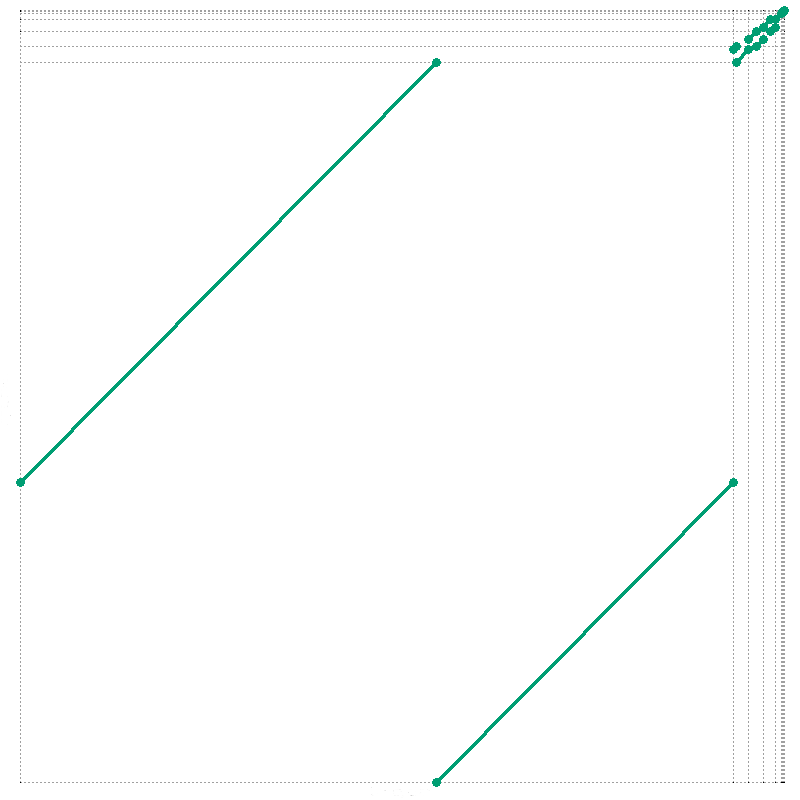
\includegraphics[width=.45\textwidth]{images/dp_c_freundii_cav1374.png}
}
\hfill
\subfloat[\emph{Klebsieall~oxytoca} CAV1015]{
	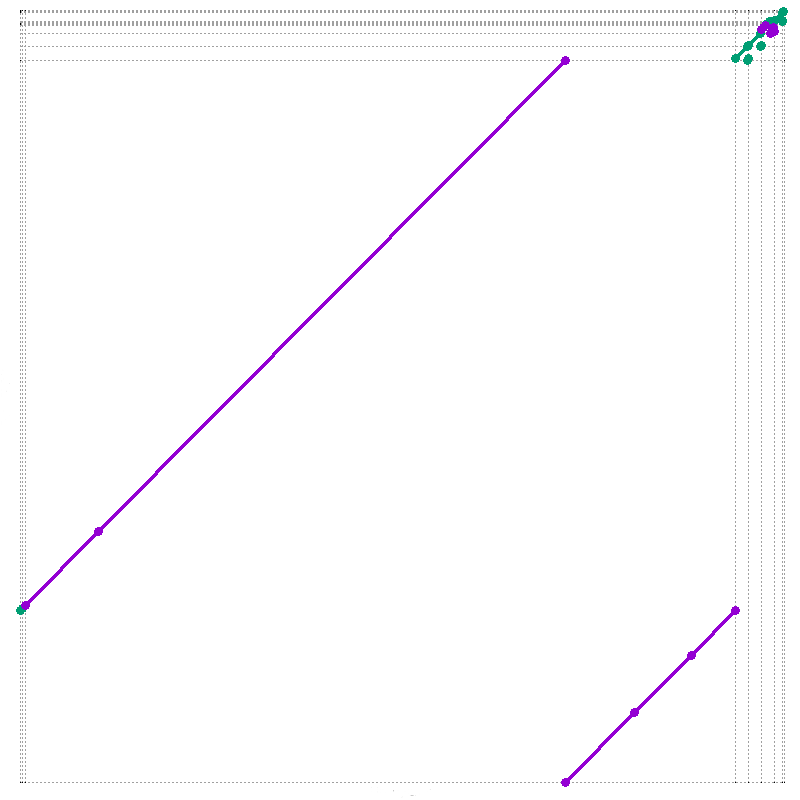
\includegraphics[width=.45\textwidth]{images/dp_k_oxytoca_cav1015.png}
}
\\
\subfloat[\emph{Enterobacter~cloacae} CAV1411]{
	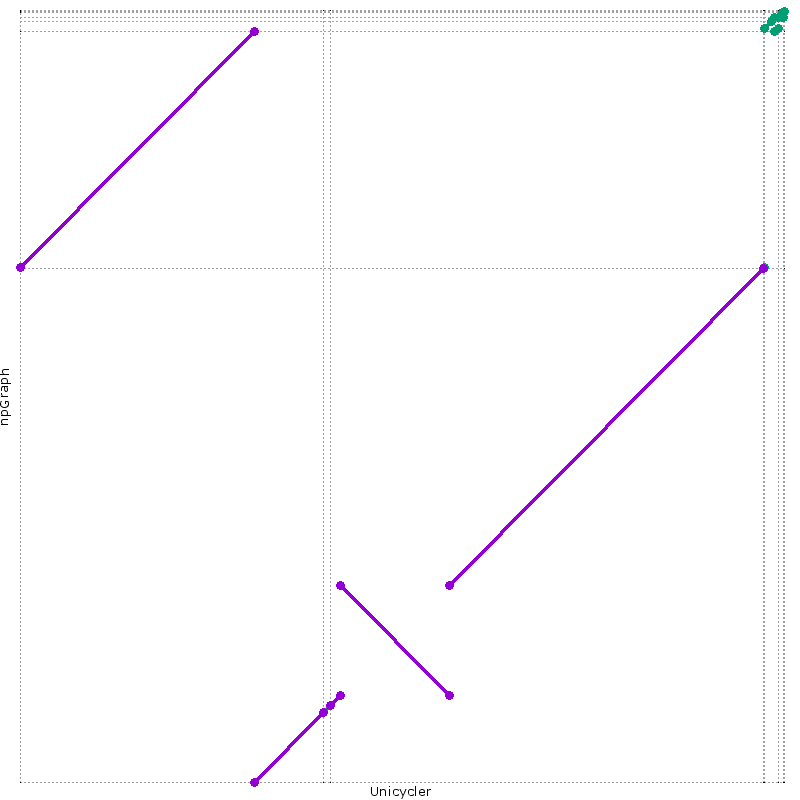
\includegraphics[width=.45\textwidth]{images/dp_e_cloacae_cav1411.png}
}
\caption[Dotplot generated by MUMmer for assembly results of \unicycler{} versus \npgraph{}.]{Dotplot generated by MUMmer for assembly results of \unicycler{} versus \npgraph{}. Structural agreements between two methods were found in (a)~\emph{C.freundii} and (b)~\emph{K.oxytoca} assembly contigs. On the other hand, for (c)~\emph{E.cloacae} sample, there was a disagreement detected between 2 largest contigs given by two assembly algorithms. This case is investigated more thoroughly by using a reference from a same bacterial strain in Figure~\ref{supp_fig:npgraph_ref}.}
\label{supp_fig:npgraph_dotplot}
\end{figure}

\begin{figure}[!hpt]
\centering
\subfloat[\emph{E.~cloacae} \unicycler{} assembly versus reference genome]{
	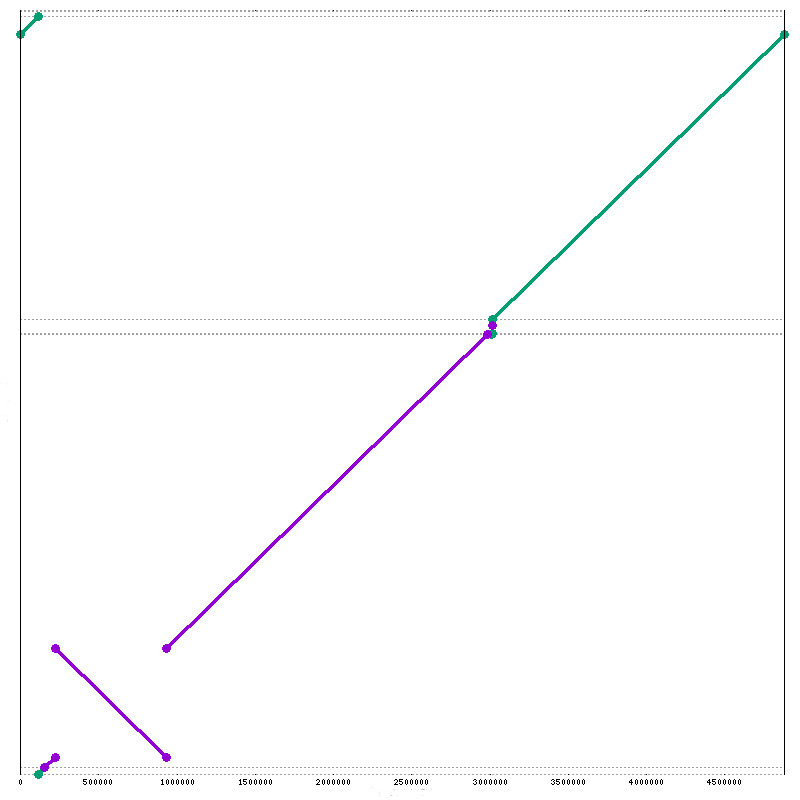
\includegraphics[width=.5\textwidth]{images/dp_ref_unicycler.png}
}
\hfill
\subfloat[\emph{E.~cloacae} \npgraph{} assembly versus reference genome]{
	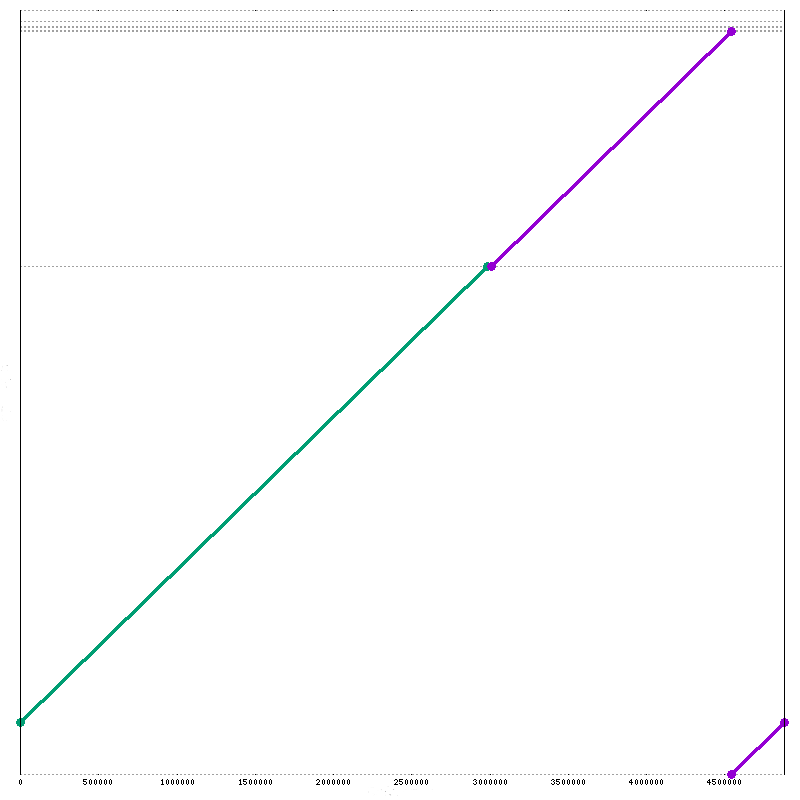
\includegraphics[width=.5\textwidth]{images/dp_ref_npgraph.png}
}
\caption[Alignments of a \emph{Enterobacter~cloacae} reference genome to assembly sequences generated by \unicycler{} and \npgraph{}]{Alignments of an \emph{Enterobacter~cloacae} reference genome to assembly sequences generated by  (a)~\unicycler{} and (b)~\npgraph{}. While the former presents a structural variant, the latter is virtually an 1-to-1 mapping.}
\label{supp_fig:npgraph_ref}
\end{figure}

\end{document}
